%%%%%%%%%%%%%%%%%%%%%%%%%%%%%%%%%%%%%%%%%%%%%%%%%%%%%%%
% A template for Wiley article submissions.
% Developed by Overleaf. 
%
% Please note that whilst this template provides a 
% preview of the typeset manuscript for submission, it 
% will not necessarily be the final publication layout.
%
% Usage notes:
% The "blind" option will make anonymous all author, affiliation, correspondence and funding information.
% Use "num-refs" option for numerical citation and references style.
% Use "alpha-refs" option for author-year citation and references style.

\documentclass[alpha-refs]{wiley-article}
% \documentclass[blind,num-refs]{wiley-article}

% Add additional packages here if required
\usepackage{siunitx}

% Update article type if known
\papertype{Original Article}
% Include section in journal if known, otherwise delete
\paperfield{Journal Section}

\title{Land-Sea Breeze Forecast Verification}

% Include full author names and degrees, when required by the journal.
% Use the \authfn to add symbols for additional footnotes and present addresses, if any. Usually start with 1 for notes about author contributions; then continuing with 2 etc if any author has a different present address.
\author[1]{Ewan Short}
\author[2]{Ben Price}
\author[3]{Derryn Griffiths}
\author[3]{Michael Foley}
%\author[2\authfn{2}]{Author Three PhD}
%\author[2]{Author B.~Four}

%\contrib[\authfn{1}]{Equally contributing authors.}

% Include full affiliation details for all authors
\affil[1]{ARC Centre of Excellence for Climate Extremes, School of Earth Sciences, University of Melbourne, Parkville, VIC, 3010, Australia}
\affil[2]{Bureau of Meteorology, Casuarina, NT, 0810, Australia}
\affil[3]{Bureau of Meteorology, Melbourne, VIC, 3208, Australia}

\corraddress{Ewan Short, ARC Centre of Excellence for Climate Extremes, School of Earth Sciences, University of Melbourne, Parkville, VIC, 3010, Australia}
\corremail{ewan.short@unimelb.edu.au}

%\presentadd[\authfn{2}]{Department, Institution, City, State or Province, Postal Code, Country}

\fundinginfo{ARC Centre of Excellence for Climate System Science}

% Include the name of the author that should appear in the running header
\runningauthor{Ewan Short et al.}

\begin{document}

\maketitle

\begin{abstract}
This study presents a methodology for comparing the performance of Australian Bureau of Meteorology forecasts of the land-sea breeze with unedited model guidance products, such as those of the European Center for Medium-Range Weather Forecasting (ECMWF) and the Australian Community Climate and Earth System Simulation (ACCESS). The methodology is applied to the 8 Australian capital city airports. The results indicate that at some airports, human intervention to model guidance products adds value to land-sea breeze forecasts, whereas at other airports it does not. 

% Please include a maximum of seven keywords
\keywords{land-sea breeze, forecast verification, Australia, Airports}
\end{abstract}

\section{Introduction}\label{introduction}
Modern weather forecasts are produced by models in conjunction with human forecasters. For instance, a forecaster working for the Australian Bureau constructs a seven day forecast by first loading model data into the Graphical Forecast Editor (GFE) software package, then manually editing this model data as they see fit. Forecasters can choose which model they wish to use, and refer to this as a choice of \textit{model guidance}. Edits are typically made to account for processes that are underesolved at synoptic scale model resolutions, or to address known biases of the models being used. 

It is therefore important to assess not only the overall accuracy of weather forecasts, but also the contribution human forecaster edits make to this accuracy. If effective, but routine, editing procedures can be identified they can be automated, freeing forecasters up to focus on other tasks. One common edit involves changing the surface wind fields near coastlines to try to represent sea-breezes more realistically than how they are resolved in the model guidance. Forecasters invest time in making sea-breeze edits because accurate predictions of near-surface winds are highly valued by a number of users, such as the aviation and energy \citep{smith09} industries. Accurate sea-breeze forecasts are also valuable to environmental monitoring authorities, as these winds provide ventilation to urban coastal areas. 

Assessing the accuracy of forecaster sea-breeze edits is more difficult than it might initially seem. Even assessing the overall accuracy of wind forecasts is not straightforward:  dozens of metrics exist, all with advantages and disadvantages \citep{mason08}. To date, previous work has focused on wind forecast verification at daily or weekly timescales \citep[e.g.][]{pinson12, lynch14}, rather than on the hourly timescale necessary for assessing land-sea breeze accuracy. Furthermore, no previous published work has attempted to assess the additional accuracy gained from forecaster wind edits seperately from the accuracy of the overall wind forecast.   

The study has two goals. First, to describe a methodology for comparing human edited forecasts of the land-sea breeze to unedited model guidance forecasts, in order to assess where and when human edits are producing an increase in accuracy. Second, to apply this methodology to the seven Australian capital city airports, which are close enough to coasts to be affected by sea-breeezes to varying degrees. The remainder of this paper is organised as follows. Section \ref{methods} describes the methodology in detail, section \ref{results} provides results, and sections \ref{discussion} and \ref{conclusion} provide a discussion and a conclusion, respectively.     

\section{Data and Methods} \label{methods}
This study compares both edited and non-edited Australian Bureau of Meteorology forecast data with automatic weather station (AWS) data from 13 Australian coastal airports. The comparison is performed by first isolating the diurnal signals of each dataset, then comparing these signals on an hour-by-hour basis. 

\subsection{Data} 
Four datasets are considered in this study; they are the Australian Bureau of Meteorology's Official wind forecast data, model data from the European Center for Medium Range Weather Forecasting (ECMWF), model data from the Australian Community Climate and Earth System Simulator (ACCESS), and observational data from automatic weather stations. The Official, ECMWF and ACCESS data are at a XX, XX degree spatial resolution respectively. Official, ACCESS and AWS data exists at each UTC hour. ECMWF data exists at a three hour resolution. To be consistent with the other data sets, ECMWF is therefore linearly interpolated to an hourly resolution: this is also what happens in practice when forecasters load ECMWF wind data into the GFE. Two time periods are considered, the austral summer months (December, January, February) of 2017/18, and the austral winter months (June, July, August) of 2018. 

Only station data from the seven Australian capital city airport automatic weather stations are considered; Official, ECMWF and ACCESS  data is \textit{(linearly?)} interpolated to the coordinates of the airport weather stations. Capital city airports have been chosen as the focus of this study for a number of reasons. Automatic weather stations located at airports tend to provide the most accurate wind data, and wind forcasts at airports are important to the aviation industry. Moreover, the capital city airports are all reasonably close to coastlines, resulting in a clear diurnal signal. Finally, these airports are also all close to their respective capital cities, which are high priority regions for accurate forecasting. The datasets are hosted on the Bureau's Jive database, but are not currently generally available, although the long term plan is for this to change. \textit{Can I extract and host the data I need myself? Can I obtain copies of the relevant Jive Functions so that I can post complete code online?}

As described above, the Australian Bureau of Meteorology's official wind forecast is constructed out of model data, which is then edited by human forecasters using the Graphical Forecast Editor (GFE) software package. Australian forecasters typically construct wind forecasts out of model data either from the European Center for Medium Range Weather Forecasting (ECMWF), or the Australian Community Climate and Earth System Simulator (ACCESS). Testing whether the official forecast data conforms more closely to the AWS observations than ECMWF or ACCESS therefore provides a way to assess the extra accuracy gained by forecaster edits.

\subsection{Assessing Diurnal Cycles}
Although close to coastlines the land-sea breeze is generally the dominant diurnal wind process, the overall diurnal signal may also include mountain-valley breezes, boundary layer mixing processes, atmospheric tides, and urban heat island circulations. Forecasters typically edit model output to account for \emph{both} unresolved sea-breezes \emph{and} unresolved boundary layer mixing; attempting to focus solely on sea-breezes without examining the entire diurnal cycle may therefore risk erroneous conclusions, with the effect of one process mistaken for another.

Sea-breezes are therefore analysed by examining the overall diurnal signal in each dataset, with the assumption that close to coastlines the land-sea breeze is the dominant diurnal process. The diurnal signal is identified by subtracting a twenty hour centred running mean \textit{background wind} from each zonal and meridional hourly wind data point. This provides a collection of zonal and meridional wind \emph{perturbation} datasets. Note that thinking of land-sea breezes in terms of perturbations from a background wind may require a conceptual shift from the usual operational definitions. A forecaster would likely define a sea-breeze to be a reversal in wind direction from a primarily offshore flow during the night and morning, to an onshore flow in the afternoon and evening. However, even if the wind is offshore the entire day, sea-breeze \emph{perturbations} are generally still detectable as a weakening of the offshore flow throughout the afternoon and evening.

Once the wind perturbation datasets have been constructed, the accuracy of the Official, ACCESS and ECMWF diurnal cycles are quantified by first calculating the Euclidean distances of the perturbations at each hour from the correspoding AWS perturbations. For instance, to quantify how closely the Official forecast perturbations match the AWS observations, we calculate the Euclidean distances $\left\lvert \boldsymbol{u}_{\text{AWS}}-\boldsymbol{u}_{\text{O}} \right\rvert$ at each time step. The accuracy with which the Official and ACCESS datasets resolve the diurnal cycle can then be compared by defining the \textit{Wind Perturbation Index} (WPI) 
\begin{equation}
\text{WPI}_\text{O,A} \equiv \left\lvert \boldsymbol{u}_{\text{AWS}}-\boldsymbol{u}_{\text{A}} \right\rvert - \left\lvert \boldsymbol{u}_{\text{AWS}}-\boldsymbol{u}_{\text{O}} \right\rvert.
\end{equation} 
At a given time, the Official forecast wind perturbation is closer to the AWS perturbation than that of ACCESS if and only if $\text{WPI} > 0$. To asses which of the Official or ECMWF forecasts are, in general, most accurate, we then take means of the WPI on an hourly basis; i.e.~all the 00:00 UTC WPI values are averaged, all the 01:00 UTC values are averaged, and so forth. The sampling distributions of these means can then be modelled as Student's $t$-distributions, and from this we can calculate the probability that $\overline{\text{WPI}} > 0$ at each hour.  

The advantage of this method is it's clarity and simplicity: we are essentially just comparing the magnitudes of vectors, then applying a two sided $t$-test to determine whether one dataset's diurnal cycle is consistently closer to observations than another's. One factor that complicates interpretation of statistics of WPI, is that the near surface winds observed in AWS data are consistenty noisier than those of the Official, ECMWF and ACCESS forecasts. This is likely due to unresolved subgrid scale turbulence in the Official, ECMWF and ACCESS model datasets. It would be unreasonable to expect forecasters to be able to predict this essentially random additional observed variability, and so a direct comparison of observed and modelled diurnal cycles may be overly stringent. 

In line with the ``fuzzy verification" agenda \citep{ebert08}, we may instead compare spatial or temporal averages of the given quantities to reduce the significance of unpredictable noise. These comparisons have less operational significance - people generally care how well the actual weather forecast performed, not whether the average of a predicted quantity matched the average of an observed quantity. However, comparisons of averages arguably better represent what we can realistically expect from human forecaster edits, and from weather forecasts overall, particularly in regards to small scale processes like sea-breezes.

\subsection{The Climatological Wind Perturbation Index}\label{climatological-performance}
Although the above methodology is perhaps the most relevant for assessing forecast performance in an operational sense, it is also informative to think about how well each forecast product performs in a
climatological sense, i.e to ask how well the \emph{mean} forecast perturbation winds match the \emph{mean} observed perturbations over a suitable climatological period. One reason for doing this is that the diurnal signal becomes much clearer when perturbations are averaged over a number of days and random variability is smoothed out. If the goal is to assess how forecasts and models capture \emph{regular} diurnal wind processes like land-sea breezes that occur at roughly the same times each day, then comparing perturbation climatologies is arguably a better option: comparing perturbations on a day to day basis will also implicitly assess how different datasets resolve \emph{irregular} processes at daily and shorter timescales; for instance turbulence and cold pool dynamics.

To assess performance on a climatological basis, steps 2 and 3 above are modified as follows. 
\begin{enumerate}
\setcounter{enumi}{1}
\item
Average the perturbations at each hour across the climatological period, i.e average all the 00:00 UTC perturbations, all the 01:00 UTC perturbations, and so forth. Calculate the quantity
\begin{equation}
\text{CWPI}_{\text{off}} \equiv \left\lvert \overline{\boldsymbol{u}}_{\text{obs}}-\overline{\boldsymbol{u}}_{\text{off}} \right\rvert.
\end{equation}
This represents the magnitude of the vector difference between the \emph{mean} 
observed wind perturbations and \emph{mean} official forecast wind perturbations. Calculate \(\text{CWPI}_{\text{mod}}\) analogously and define the the \emph{Climatological Wind Perturbation Index}
\begin{equation}
\text{CWPI} = \text{CWPI}_{\text{mod}} - \text{CWPI}_{\text{off}}.
\end{equation}
\item
Estimate the sampling distribution of \(\text{CWPI}\) by bootstrapping
\citep{efron79}. Use the sampling distribution to calculate the likelihood that $\text{CWPI} > 0$.  
\end{enumerate}

Although they have similar definitions, $\overline{\text{WPI}}$ and CWPI measure different things. They do not converge as the length of the time period grows - they don't even necessarily approach the same sign. As a simple example, suppose that for each day, the observed and Official wind perturbations are given by $\boldsymbol{p}_{\text{AWS}} = \left(5\cos\omega t , 5\sin\omega t\right)$ and $\boldsymbol{p}_\text{O} = \left(6\cos\omega t , 6\sin\omega t\right)$, respectively. Furthermore, suppose that the ACCESS perturbations alternate between $\boldsymbol{p}_{\text{A}} = \left(7\cos\omega t , 7\sin\omega t\right)$ and $\boldsymbol{p}_{\text{A}} = \left(3\cos\omega t , 3\sin\omega t\right)$ from one day to the next. Then for any contiguous period of $n$ days, $\overline{\text{WPI}} = 2 - 1 = 1$, but $\text{CWPI} \approx -1$, with the approximation becoming exact for even $n$. Moreover $\overline{\text{WPI}}=1$ with a confidence of 1, and using the bootstrapping procesure described above, the confidence that $\text{CWPI} = -1$ approaches 1 as $n\to \infty$. This example shows that while the WPI and CWPI are sensitive both to random error and consistent biases between the different datasets, the CWPI becomes increasingly less sensitive to random error as the length of the time period being considered grows. Thus while the WPI arguably provides a more meaningful operational metric, as it measures the accuracy of actual forecast data, it may favour a more biased dataset over a less biased one, just because the internal variability of that dataset is lower. One consequence of this is that model data at a lower spatiotemporal resolution may outperform in $\overline{\text{WPI}}$ model data of a higher resolution, purely because the internal variability is lower. In this way, the CWPI may actually provide more information about the performance of different forecasts.

\begin{enumerate}
\item
Note that the Bureau has not yet moved to ensemble forecasting - and probabilistic forecasting methods therefore not appropriate. 
\end{enumerate}

\section{Results}
\label{results}

\begin{enumerate}
\item
Example figure with one day diurnal cycles for both AWS, Official, ECMWF and ACCESS winds, perturbations, and perturbation climatology. Just one season.
\item
Airport breakdown for one season, WPI, CWPI for one season, for both ACCESS and ECMWF. Second season in online supporting material.
\item
Example results for straight coastlines - perhaps north, northeast, northwest, south, southeast, southwest? Again, just do one season, include second season in online supporting material?
\item
Look at timing results by fitting ellipses and checking orientations of major axes. Just one season - both ECMWF and ACCESS? Maybe just ACCESS if ECMWF results are dodgy?
\end{enumerate}

\begin{enumerate}
\item
In Cairns and Townsville (austral summer), ECMWF understimates the magnitude of the land-sea breeze, leading to ACCESS resolving the diurnal cycle more accurately. During austral winter ECMWF again underperfoms, but (Townsville) more to do with shape of the hodograph and direction of the sea-breeze. At Cairns, it's essentially again because the ECMWF peak seabreeze is slightly (1 knot) too slow.   
\item
In Darwin - ACCESS perturbations bizarre during austral summer (wet season), but ECMWF also much too weak (about half the amplitude). 
\item
In Darwin - during austral winter (dry season) - ECMWF very accurate - gets peak of sea-breeze perfectly correct! Also resolves weird bump at 12 UTC quite well. However, does not resolve bump at 1 UTC at all. ACCESS doesn't either really. 
\item
Interesting - at Melbourne ECMWF and ACCESS essentially agree, but both underestimate the magnitude of the land-sea breeze. True of both seasons. 
\item
Adelaide - ACCESS and ECMWF almost match at Adelaide. Amplitudes generally slightly too weak compared to observations however. 
\item
Need to assume intependence of measurement and rounding error in observations. 
\end{enumerate}

\begin{figure}
\centering
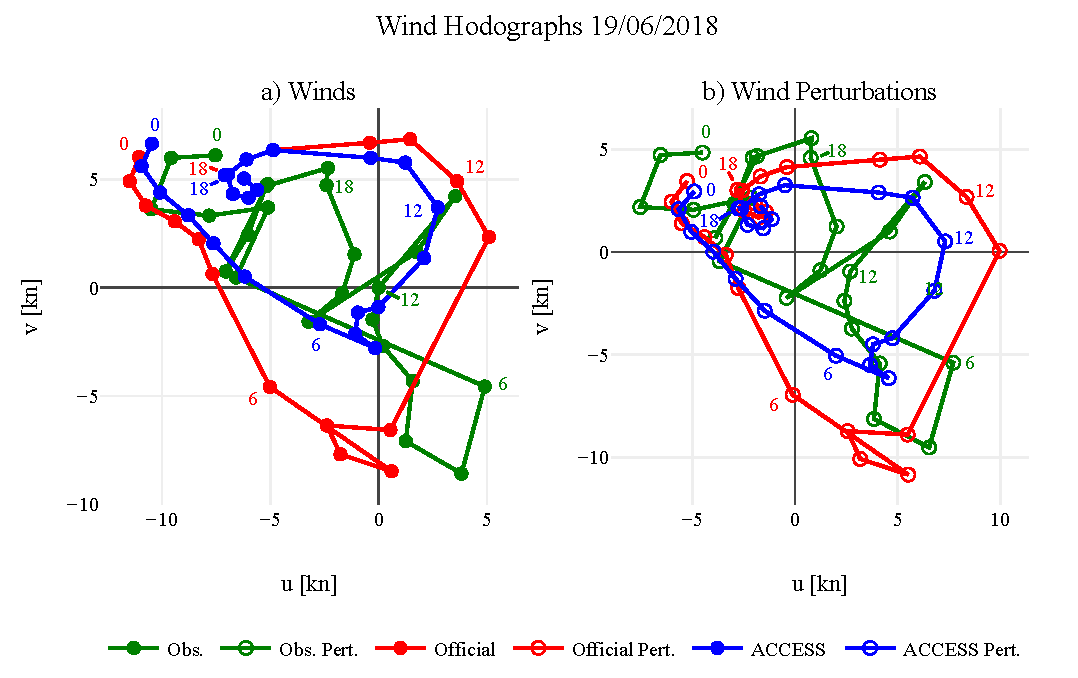
\includegraphics[keepaspectratio=true, height=7cm]{daily_winds_darwin_AP.pdf}
\caption{Hodographs showing the a) winds and b) wind perturbations (from a 24-hour running mean) at each hour [UTC] on 19/06/2018 at Darwin Airport.}
\label{Fig:airport_wpi_access}
\end{figure}

\begin{figure}
\centering
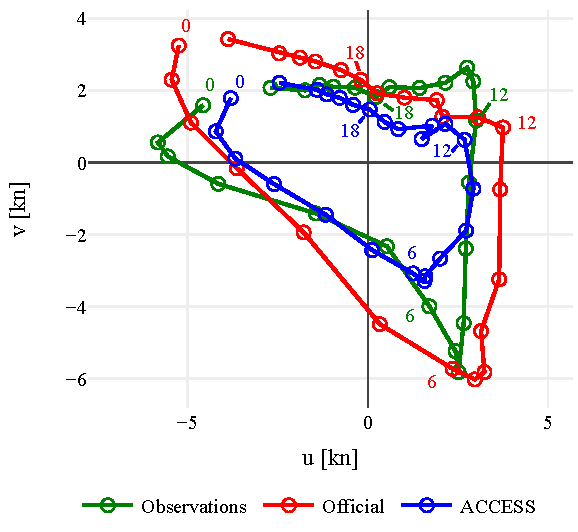
\includegraphics[keepaspectratio=true,height=7cm]{clim_winds_austral_winter_ACCESS.pdf}
\caption{Hodograph showing the wind perturbations (from a 24-hour running mean) at each hour [UTC] at Darwin Airport, averaged across June, July, August 2018.}
\label{Fig:airport_wpi_access}
\end{figure}

\begin{figure}
\centering
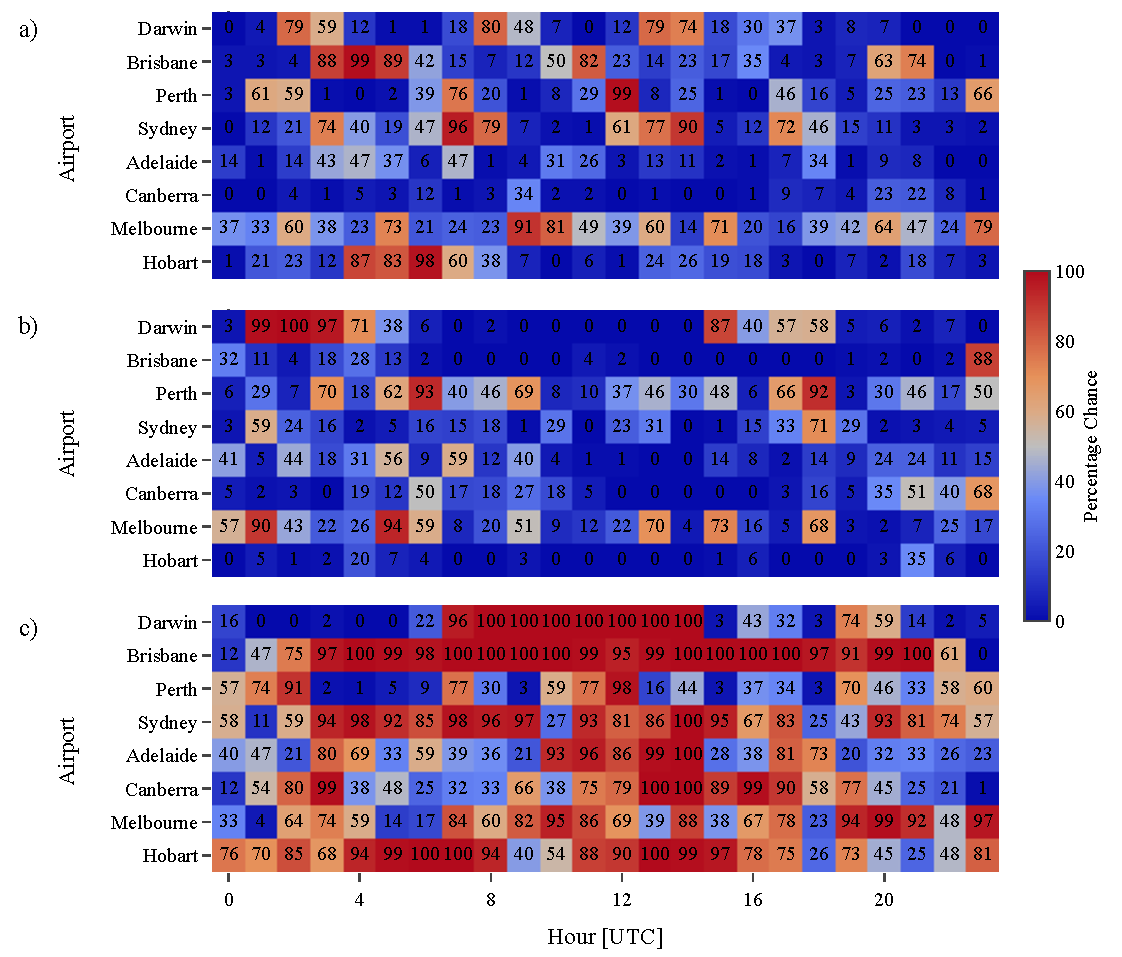
\includegraphics[keepaspectratio=true,width=0.90\textwidth]{airport_wpi_winter.pdf}
\caption{Confidence that a) the Bureau's official forecasts of diurnal wind processes are more accurate than unedited ACCESS model guidance over the austral winter months (June, July, August) of 2018, as measured by the WPI; analogously, b) and c) give the confidence that the Official forecast is more accurate than ECMWF model guidance, and that ECMWF is more accurate that ACCESS, respectlvely. }
\label{Fig:airport_wpi_access}
\end{figure}

\begin{figure}
\centering
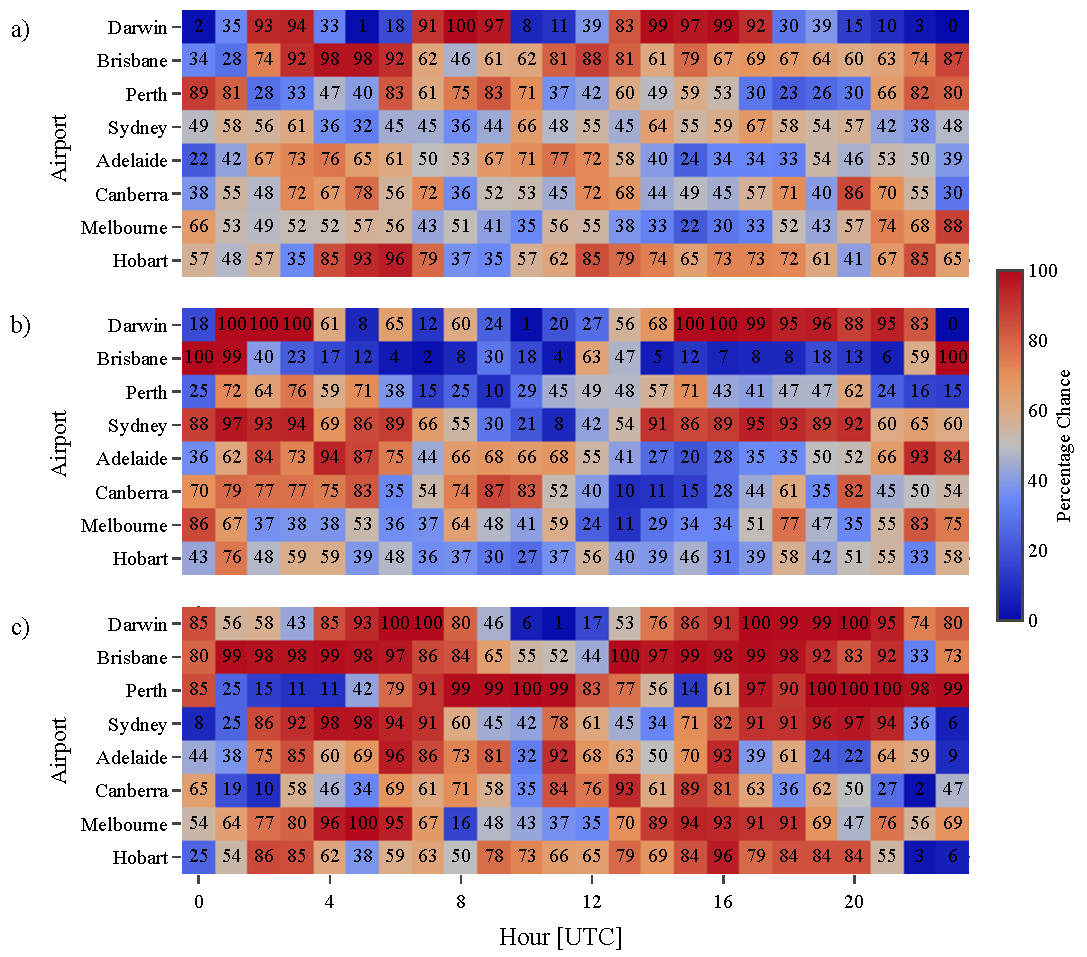
\includegraphics[keepaspectratio=true,width=0.90\textwidth]{airport_cwpi_winter.pdf}
%\caption{As in Fig.~\ref{Fig:airport_wpi_access}, but measured using the CWPI.}
\label{Fig:airport_cwpi_access}
\end{figure}

\section{Discussion}
\label{discussion}

The methods developed in this study can be readily extended to analyse \emph{just} the sea-breezes satisfying the operational definition above. For instance, to study the sea-breezes at a station near a coastline with inward pointing normal vector $\widehat{\boldsymbol{n}}$, the wind perturbation datasets could be restricted to just those days where the corresponding raw wind vector $\boldsymbol{u}$ satisfies $\widehat{\boldsymbol{n}} \cdot \boldsymbol{u} > 0$ for at least one of the hours of that day.

\subsection{\citet{pinson12}}
Proposes station-oriented view of the verification problem (which is what we are doing). Notes that there is a ``representativeness issue" in that station-data is resolving processes at physical scales the model is infact not intended to resolve. Notes that from the users perspective this is irrelevant. \textit{How could forecasters or post-processing incorporate this uncertainty into the forecast?} Discusses in detail the bilinear interpolation process for downscaling forecast data to location of stations. \textit{What is Jive's procedure for doing this?} Forecasts are benchmarked against 1-6 climatology based forecasts. Notes that observational uncertainty is known to be non-negligible, while surface effects introduce additional noise beyond what the numerical models intend to represent (or are capable of representing.) Representativeness issue ignored here for above reasons. Notes one method of dealing with observational uncertainty when performing ensemble (probabilistic) forecast verification is by transforming observations into random variables. Impact of observational uncertainty can then be assessed using methods like those of Pappenberger et al.~(2009). Note that Pappenberger still applies only to probabilistic forecasting. 

Very important - notes that the most poorly performing locations across Europe are the Alps and coastal regions, and that ``This could be expected since near-surface local effects [e.g. mountain and sea-breezes] are difficult to resolve at the fairly coarse resolution (50 km) of the ECMWF ensemble prediction system. [What is the spatial resolution of the ECMWF, ACCESS data used in GFE?] Authors comment on ``...questionable quality of the ensemble forecasts, for instance due to local effects not represented in a model with such a coarse spatial resolution". Could also be ensemble averaging process suppressing local processes.    

Key discussion - ``The periodic nature of the RMSE curves is linked to the diurnal cycles in the wind speed magnitude, the amplitude of such periodicities varying throughout Europe. To identify better the effect of the diurnal cycle on verification statistics, one may refine the analysis performed here by verifying forecasts depending on the time of the day (instead of the lead time), or by making a difference between forecasts issued at 0000 and 1200 UTC." So diurnal cycles are mentioned in passing here - good reference to make.  

Regarding observational uncertainty - the effect of uncertainty diminishes as the number of stations or the length of the evaluation period increases. ``This effect was observed to become negligible if looking at more than 100 stations over periods of more than a month (with two forecast series issued per day). For certain sites with strong local regimes though, one retrieves a more intuitive result that ensembles significantly underestimate wind speed.  

\subsection{\citet{lynch14}}
Focuses more on longer term forecasts. Interesting note that there is little difference in performance between 10m and 100m winds. Applies verification to forecast anomalies (from seasonal and diurnal cycles). SImilar approach to me, but work out average for each hour for each day of year, averaged over 32 years of ERA-Interim record. Note that I'm also avoiding the ``aritificial skill" associated with the seasonal cycle by restricting to just a particular season. I'm not convinced that seasonal skill is necessarily ``artificial" however! Both pinson and lynch use the CPRS score. Interesting notes on the large costs associated with wind farm station maintenance, and the need for probabilistic forecasts in order to manage these costs. 

\subsection{\citet{ebert08}}
Not easy to prove the value of mesoscale forecasts using traditional point-by-point verification results. At small scale features unpredictable - e.g. intermittant convective rainfall - in the example of winds the cold pool dynamics. Mesoscale forecasts typically verified against high-resolution gridded datasets, e.g. radar mosaics or reanalysis. Spatial verification techniques that do not require the forecasts to exactly match the observations at fine scales. Use of ``object oriented" techniques. The term `fuzzy' is consistent with the general concept of 'partial truth' introduced by Zadeh. Does Ebert's fuzzy scheme require gridded data? No. ``Fuzzy verification assumes that it is acceptable for the forecast to be slightly displaced and still be useful. Fuzzy concept can be applied in space or time. Really we're doing ``upscaling" rather than ``fuzzy" verification. Uncertainty in the observations represented by using neighbouring grid boxes. Less useful to me because ``event" framework not entirely appropriate to diurnal cycles. I am using an ``upscaling" approach. ``From the perspective of the forecast user, fuzzy verification gives important information on the scales and intensities at which the forecasts should be trusted." 

\subsection{\citet{yates06}}

\section{Conclusion}
\label{conclusion}
In this report, a methodology for comparing the performance of Bureau forecasts of diurnal wind processes to unedited model guidance products has been developed and applied to a case study of the Darwin airport. The key results may be summarised as follows.
\begin{enumerate}
\item
During the dry season months of June, July and August 2017, the ECMWF sea-breeze is generally more accurate than that of the official forecast. However, during the wet season months of December, January and February 2017/18 this result is reversed, and the official forecast sea-breeze generally outperforms that of ECMWF. 
\item
In both seasons, boundary layer mixing processes are generally represented better in official forecasts than in ECMWF.
\item
In the dry season, the climatological wind perturbations of the official forecast generally outperform those of ECMWF between 13:00 and 16:00 UTC. This is due to ECMWF not capturing the magnitude of the south-easterly mean perturbations. 
\item
During the wet season, the climatological wind perturbations of the official forecast generally outperform those of ECMWF at 11:00 UTC. This is due to ECMWF underestimating the magnitude of the mean land-breeze perturbation.
\end{enumerate}    

There a number of ways that this work could be extended. The most pressing would probably be to investigate whether the results presented here change when a more operational definition of the sea breeze is used in place of the entirely perturbation based definition used here: this could be done using the method described in section \ref{methods}.

Following this, a nationwide study could be conducted focusing on the most operationally relevant locations of each state, for instance, airport stations. This should be done on a seasonal basis given that the examples considered here indicate results are seasonally dependent. The boundary layer mixing and sea-breeze editing techniques used by forecasters could then be collated and compared, with a view to standardising them across the country and optimising performance.

\bibliography{./Coastal_Winds.bib}

\end{document}
